\documentclass[12pt]{article}
\usepackage[utf8]{inputenc}
\usepackage{geometry}
\geometry{letterpaper, margin=0.25in}
\usepackage{graphicx} 
\usepackage{parskip}
\usepackage{booktabs}
\usepackage{array} 
\usepackage{paralist} 
\usepackage{verbatim}
\usepackage{subfig}
\usepackage{fancyhdr}
\usepackage{sectsty}
\usepackage[shortlabels]{enumitem}

\pagestyle{fancy}
\renewcommand{\headrulewidth}{0pt} 
\lhead{}\chead{}\rhead{}
\lfoot{}\cfoot{\thepage}\rfoot{}

%%% ToC (table of contents) APPEARANCE
\usepackage[nottoc,notlof,notlot]{tocbibind} 
\usepackage[titles,subfigure]{tocloft}
\renewcommand{\cftsecfont}{\rmfamily\mdseries\upshape}
\renewcommand{\cftsecpagefont}{\rmfamily\mdseries\upshape} %

\usepackage{amsmath}
\usepackage{amssymb}
\usepackage{mathtools}
\usepackage{empheq}
\usepackage{xcolor}
\usepackage{bbm}
\usepackage{tikz}
\usepackage{pgfplots}
\usepackage{tikz-cd}
\pgfplotsset{compat=1.18}
\usetikzlibrary{intersections, decorations.markings}
\tikzset{
    marking along/.style n args={2}{
        decoration={
                markings, 
                mark=at position #1 with {\arrow{#2}}
        },
        postaction={decorate}
        },
    marking along/.default={0.5}{>}
}

\newcommand{\ans}[1]{\boxed{\text{#1}}}
\newcommand{\vecs}[1]{\langle #1\rangle}
\renewcommand{\hat}[1]{\widehat{#1}}

\renewcommand{\P}{\mathbb{P}}
\newcommand{\R}{\mathbb{R}}
\newcommand{\E}{\mathbb{E}}
\newcommand{\Z}{\mathbb{Z}}
\newcommand{\N}{\mathbb{N}}
\newcommand{\Q}{\mathbb{Q}}
\newcommand{\C}{\mathbb{C}}

\newcommand{\ind}{\mathbbm{1}}
\newcommand{\qed}{\quad \blacksquare}

\newcommand{\brak}[1]{\left\langle #1 \right\rangle}
\newcommand{\bra}[1]{\left\langle #1 \right\vert}
\newcommand{\ket}[1]{\left\vert #1 \right\rangle}

\newcommand{\abs}[1]{\left\vert #1 \right\vert}
\newcommand{\mfX}{\mathfrak{X}}
\newcommand{\ep}{\varepsilon}

\newcommand{\Ec}{\mathcal{E}}
\newcommand{\Nc}{\mathcal{N}}
\newcommand{\A}{\mathcal{A}}
\newcommand{\F}{\mathcal{F}}
\newcommand{\Cc}{\mathcal{C}}
\newcommand{\B}{\mathcal{B}}
\newcommand{\M}{\mathcal{M}}
\newcommand{\X}{\chi}
\renewcommand{\L}{\mathcal{L}}

\newcommand{\sub}{\subseteq}
\newcommand{\st}{\text{ s.t. }}
\newcommand{\card}{\text{card }}
\renewcommand{\div}{\vspace*{10pt}\hrule\vspace*{10pt}}
\newcommand{\surj}{\twoheadrightarrow}
\newcommand{\inj}{\hookrightarrow}
\newcommand{\biject}{\hookrightarrow \hspace{-8pt} \rightarrow}
\renewcommand{\bar}[1]{\overline{#1}}
\newcommand{\overcirc}[1]{\overset{\circ}{#1}}
\newcommand{\diam}{\text{diam }}
\newcommand{\iid}{\overset{	ext{iid}}{\sim}}

\renewcommand{\Re}{\text{Re}\,}
\renewcommand{\Im}{\text{Im}\,}
\newcommand{\Var}{\text{Var}\,}
\newcommand{\Cov}{\text{Cov}\,}

\DeclareMathOperator*{\argmax}{\arg\max}
\DeclareMathOperator*{\argmin}{\arg\min}

\newcommand{\sign}{\text{sign}\,}

\newcommand*{\tbf}[1]{\ifmmode\mathbf{#1}\else\textbf{#1}\fi}

\usepackage{tcolorbox}
\tcbuselibrary{breakable, skins}
\tcbset{enhanced}
\newenvironment*{tbox}[2][gray]{
    \begin{tcolorbox}[
        parbox=false,
        colback=#1!5!white,
        colframe=#1!75!black,
        breakable,
        title={#2}
    ]}
    {\end{tcolorbox}}

\newenvironment*{exercise}[1][red]{
    \begin{tcolorbox}[
        parbox=false,
        colback=#1!5!white,
        colframe=#1!75!black,
        breakable
    ]}
    {\end{tcolorbox}}

\newenvironment*{proof}[1][blue]{
\begin{tcolorbox}[
    parbox=false,
    colback=#1!5!white,
    colframe=#1!75!black,
    breakable
]}
{\end{tcolorbox}}
\newenvironment*{proposition}[1][gray]{
    \begin{tcolorbox}[
        parbox=false,
        colback=#1!5!white,
        colframe=#1!75!black,
        breakable
    ]}
    {\end{tcolorbox}}

\title{APMA 1360: Homework 8}
\author{Milan Capoor}
\date{4 April 2025}

\begin{document}
\maketitle


\section{Stability}

Consider the system $\dot{u}=F(u)$ with $u\in\R^n$ and $F\in C^2$. We assume that $u=0$ is an equilibrium and that its Jacobian $A=F_u(0)$ is a diagonal matrix with entries $\lambda_1,\ldots,\lambda_n$ on the diagonal and zeros everywhere else.

I stated in class that if all eigenvalues $\lambda_1,\ldots,\lambda_n$ of $A$ have strictly negative real part, then the origin is stable. The goal of this problem is to prove this statement.
\begin{enumerate}[(i)]
    \item Assume that the eigenvalues $\lambda_1,\ldots,\lambda_n$  of the diagonal matrix $A$ are strictly negative. Show that there is a $\delta>0$ so that
          \[
              V(u) = \sum_{j=1}^n u_j^2 = |u|^2
          \]
          is a Lyapunov functional for all $u=(u_1,\ldots,u_n)\in\R^n$ with $|u|<\delta$.


          \color{blue}
          \[\nabla V(u) = \begin{pmatrix}
                  2u_1   \\
                  \vdots \\
                  2u_n
              \end{pmatrix} = 2u\]

          From the Taylor series, if $\abs{u} <  1$,
          \[\abs{F(u) - F(0) - F_u(0)u} \leq C\abs{u}^2\]
          but $F(0) = 0$ so we have
          \[\abs{F(u) - F_u(0)u} = \abs{F(u) - Au} \leq C\abs u^2\]

          Hence, it suffices to show
          \[\brak{V(u), F(u)} < 0 \iff \brak{V(u), Au + F(u) - Au} < 0 \iff 2u \cdot Au + 2u \cdot (F(u) - Au) < 0 \]

          First consider $2u \cdot Au$:
          \begin{align*}
              2u \cdot Au & = 2\sum_{j=1}^{n} u_j \lambda_j u_j                                                       \\
                          & = 2\sum_{j=1}^{n} \lambda_j u_j^2                                                         \\
                          & = 2\sum_{j=1}^n \tilde \lambda u_j^2 < 0 \qquad (\tilde \lambda := \max(\lambda_{i=1:n})) \\
                          & =2\tilde \lambda \abs{u}^2                                                                \\
                          & < 2\tilde \lambda \delta^2
          \end{align*}

          Now consider $2u \cdot (F(u) - Au) < 0$. Again by the Taylor expansion,
          \begin{align*}
              2u \cdot (F(u) - Au) & \leq 2\abs{u \cdot (F(u) - Au)} \\
                                   & = 2\abs{u}\, \abs{F(u) - Au}    \\
                                   & \leq 2C \abs{u} \abs{u}^2       \\
                                   & \leq 2C \delta^3
          \end{align*}

          So it suffices to have
          \[2\tilde \lambda \delta^2 + 2C \delta^3 < 0\]

          Since we need $0 < \abs{u} < 1$, assume $\delta < 1$, giving
          \[2\tilde \lambda \delta^2 + 2C \delta^3  < 2\tilde \lambda \delta + 2C \delta^2\]

          Requiring this to be less than zero,
          \[2\tilde \lambda \delta + 2C \delta^2 < 0 \implies \delta < -\frac{\tilde \lambda}{C} \]

          By construction, for $\delta = \min\left(1, -\frac{\max\{\lambda_1, \dots, \lambda_n\}}{C}\right)$, $V$ is a Lyapunov functional for all $u$ with $\abs{u} < \delta$.

          \color{black}
    \item In the case described in (ii), prove that the origin is stable.

          \color{blue}
          We wish to show that $\exists \delta > 0$ such that $\abs{u(0)} < \delta \implies u(t) \to 0$.

          Let $\delta$ be the same as in (i). Then, since $V$ is a Lyapunov functional, by a Lemma from class,
          \[\frac{d}{dt} V(u(t)) < 0 \implies \frac{d}{dt}\abs{u(t)}^2 < 0    \]

          But this implies that $\abs{u(t)}^2 < \abs{u(0)}^2 < \delta^2$ for all $t > 0$. Since $\abs{u(t)}^2 \geq 0$ by definition of the norm, we have that $\abs{u(t)}^2 \to 0 \implies \abs{u(t)} \to 0$ as $t \to \infty$, exactly as desired.
          \color{black}
\end{enumerate}

Here is additional information that may be useful:
\begin{itemize}
    \item  Recall that we say that an equilibrium $u_*$ is stable if there is a $\delta>0$ so that $u(t)\to u_*$ as $t\to\infty$ for all solutions $u(t)$ of $\dot{u}=F(u)$ for which $|u(0)-u_*|<\delta$. Here, $|u|$ denotes the norm of a vector in $\R^n$.
    \item You can use without proof that for each function $F\in C^2$ there is a constant $C>0$ so that
          \[
              |F(u)-F(0)-F_u(0)u| \leq C |u|^2
          \]
          for all $u$ with $|u|\leq1$. This follows from the Taylor series expansion for $F$.
\end{itemize}

\pagebreak

%%%%%%%%%%%%%%%%%%%%%%%%%%%%%%%%

\section{Lyapunov functionals}

Consider the system
\[
    \begin{pmatrix} \dot{x} \\ \dot{y} \end{pmatrix} =
    \begin{pmatrix} y-x^3 \\ -x-y^3 \end{pmatrix}
\]
\begin{enumerate}[(i)]
    \item Show that this system has a Lyapunov functional of the form $V(x,y)=ax^2+by^2$ for appropriate values of $a,b$.

          \color{blue}
          Let $F(x, y) = \begin{pmatrix} y-x^3 \\ -x-y^3 \end{pmatrix}$.

          Trivially, we have $F(x, y) = 0$ where $(x, y) = (x, x^3)$ and $(x, y) = (-y^3, y)$

          \begin{center}
              \color{black}

              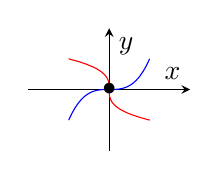
\begin{tikzpicture}
                  \begin{axis}[
                          width=0.3\textwidth,
                          axis lines=middle,
                          no markers,
                          xtick=\empty,
                          ytick=\empty,
                          clip=false,
                          xlabel={$x$},
                          ylabel={$y$},
                          domain=-1:1,
                          ymin=-2, ymax=2,
                          xmin= -2, xmax=2,
                          view = {0}{90}
                      ]
                      \addplot[name path=x, blue] {x^3};
                      \addplot[name path=y, red] ({-x^3}, {x});

                      \fill [name intersections={of=x and y, total=\t}]
                      \foreach \s in {1,...,\t}{(intersection-\s) node {$\bullet$}};
                  \end{axis}
              \end{tikzpicture}
          \end{center}

          That is, only at $(x, y) = (0, 0)$.

          We want to show that $V(x, y) = ax^2 + by^2$ is a Lyapunov functional for $F$ for all $(x, y) \neq (0, 0)$:
          \begin{align*}
              \nabla V(x, y)                 & = \begin{pmatrix}
                                                     \frac{\partial V}{\partial x} \\
                                                     \frac{\partial V}{\partial y}
                                                 \end{pmatrix} = \begin{pmatrix}
                                                                     2ax \\
                                                                     2by
                                                                 \end{pmatrix}     \\
              \brak{\nabla V(x, y), F(x, y)} & = \begin{pmatrix}
                                                     2ax \\
                                                     2by
                                                 \end{pmatrix} \cdot \begin{pmatrix}
                                                                         y-x^3 \\
                                                                         -x-y^3
                                                                     \end{pmatrix} \\
                                             & = 2a(xy-x^4) - 2b(xy+y^4)
          \end{align*}

          Hence, we need
          \[2a(xy-x^4) < 2b(xy+y^4)\]

          If $a = b > 0$,
          \[2a(xy - x^4) - 2a(xy + y^4) = -2ax^4 - 2ay^4 < 0 \quad \forall x, y\]

          Hence $V$ is a Lyapunov functional for $F$ if $a = b > 0$.

          \color{black}


    \item Use this result to show that this system cannot have any periodic orbits.

          \color{blue}
          By a Lemma from class, since $V$ is a Lyapunov functional, the system cannot have any (non-trivial) periodic orbits.
          \color{black}

\end{enumerate}

\pagebreak

%%%%%%%%%%%%%%%%%%%%%%%%%%%%%%%%

\section{Conserved systems}

Consider the second-order equation $\ddot{x}=x-x^2$.
\begin{enumerate}[(i)]
    \item Write this equation as a second-order system for $(x,\dot{x})$.

          \color{blue}
          Let $y = \dot x$. Then,
          \[\ddot x = \dot y = x - x^2\]
          so we may write
          \[\begin{pmatrix}
                  \dot x \\
                  \dot y
              \end{pmatrix} = \begin{pmatrix}
                  y \\
                  x - x^2
              \end{pmatrix} = F(x, y)\]
          \color{black}

    \item Find all equilibria.

          \color{blue}
          \[\begin{pmatrix}
                  \dot x \\
                  \dot y
              \end{pmatrix} = 0 \implies \begin{cases}
                  y = 0 \\
                  x - x^2 = 0
              \end{cases} \implies \begin{cases}
                  y = 0 \\
                  x = \{0, 1\}
              \end{cases}\]
          which means we have equilibria at $(0, 0)$ and $(1, 0)$.
          \color{black}

    \item Find a conserved quantity.

          \color{blue}
          As in class, we suspect
          \[H(x, y)  = \frac{y^2}{2} - \int_0^x t-t^2\; dt = \frac{y^2}{2} - \frac{x^2}{2} + \frac{x^3}{3}\]
          will be conserved.

          It suffices to check $\brak{\nabla H(x, y), F(x, y)} = 0$:
          \begin{align*}
              \nabla H(x, y)                 & = \begin{pmatrix}
                                                     -x + x^2 \\
                                                     y
                                                 \end{pmatrix}                \\
              \brak{\nabla H(x, y), F(x, y)} & = -(x - x^2)y + y(x -  x^2) = 0
          \end{align*}
          as desired.
          \color{black}

    \item Sketch the phase portrait.

          \begin{center}
              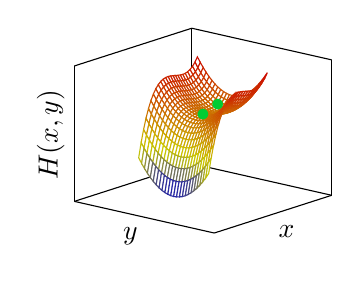
\begin{tikzpicture}
                  \begin{axis}[
                          width=0.4\textwidth,
                          %axis lines=middle,
                          no markers,
                          xtick=\empty,
                          ytick=\empty,
                          ztick=\empty,
                          clip=false,
                          xlabel={$x$},
                          ylabel={$y$},
                          zlabel={$H(x, y)$},
                          domain=-2:2,
                          ymin=-4, ymax=4,
                          xmin= -4, xmax=4,
                          view = {-50}{20}
                      ]
                      %\addplot3[mesh] {y^2/2 - x^2/2 + x^3/3};
                      \addplot3[surf, fill=white] {y^2/2 - x^2/2 + x^3/3};


                      \node[green!60!teal] at (0, 0, 0) {$\bullet$};
                      \node[green!60!teal] at (1, 0, 1/3) {$\bullet$};
                  \end{axis}
              \end{tikzpicture}
              \hspace{1cm}
              \begin{tikzpicture}
                  \begin{axis}[
                          width=0.4\textwidth,
                          axis lines=middle,
                          no markers,
                          xtick=\empty,
                          ytick=\empty,
                          ztick=\empty,
                          clip=false,
                          xlabel={$x$},
                          ylabel={$y$},
                          zlabel={$H(x, y)$},
                          domain=-2:2,
                          ymin=-2, ymax=2,
                          xmin= -2, xmax=2,
                          view = {0}{90}
                      ]

                      \addplot3[gray, quiver={u=y, v=x-x^2, scale arrows=0.1}, samples=10, -stealth] {0};
                      \addplot3[contour gnuplot ] {y^2/2 - x^2/2 + x^3/3};

                      \node[green!60!teal] at (0, 0, 0) {$\bullet$};
                      \node[green!60!teal] at (1, 0, 1/3) {$\bullet$};
                  \end{axis}
              \end{tikzpicture}
          \end{center}


\end{enumerate}



\end{document}